\section{fidanka}\label{sec:fidanka}
When fitting isochrones to the clusters with multiple populations we have four
main criteria for any method

\begin{itemize}
  \item The method must be robust enough to work along the entire main
    sequence, turn off, and much of the subgiant and red giant branch.
	\item Any method should consider photometric uncertainty in the fitting process.
	\item The method should be model independent, weighting any n number of populations equally.
	\item The method should be automated and require minimal intervention from the user.
\end{itemize}


We do not believe that any currently available software is a match for
our use case. Therefore, we elect to develop our own software suite, \fidanka.
\fidanka is a python package designed to automate much of the process of
measuring fiducial lines in CMDs, adhering to the four criteria we lay out
above. Primary features of \fidanka may be separated into three
categories: fiducial line measurement, stellar population synthesis, and
isochrone optimization/fitting. Additionally, there are utility functions that
are detailed in the \fidanka documentation.

\subsection{Fiducial Line Measurement}
\fidanka takes a iterative approach to measuring fiducial lines, the first step
of which is to make a ``guess'' as to the fiducial line. This initial guess
is calculated by splitting the CMD into magnitude bins, with uniform numbers of
stars per bin (so that bins are cover a small magnitude range over densely
populated regions of the CMD while covering a much larger magnitude range in
sparsely populated regions of the CMD, such as the RGB). A unimodal Gaussian
distribution is then fit to the color distribution of each bin, and the
resulting mean color is used as the initial fiducial line guess. This rough
fiducial line will approximately trace the area of highest density. The initial
guess will be used to verticalize the CMD so that further algorithms can work in
1-D magnitude bins without worrying about weighting issues caused by varying
projections of the evolutionary sequence onto the magnitude axis.
Verticalization is performed taking the difference between the guess fiducial
line and the color of each star in the CMD.

If \fidanka were to simply apply the same algorithm to the verticalized CMD
then the resulting fiducial line would likely be a re-extraction of the initial
fiducial line guess. To avoid this, we take a more robust, number density based
approach, which considers the distribution of stars in both color and magnitude
space simultaneously. For each star in the CMD we first use an
\texttt{introselect} partitioning algorithm to select the 50 nearest stars in
F814W vs. F275W-F814W space. To account for the case where the star is at an
extreme edge of the CMD, those 50 stars include the star itself (such that we
really select 49 stars + 1). We use
\texttt{qhull}\footnote{https://www.qhull.com}\citep{Barber1996} to calculate
the convex hull of those 50 points. The number density at each star then is
defined as $50/A_{hull}$, where $A_{hull}$ is the area of the convex hull.
Because we use a fixed number of points per star, and a partitioning algorithm
as opposed to a sorting algorithm, this method scales like $\mathcal{O}(n)$,
where n is the number of stars in the CMD. This method also intrinsically
weights the density of of each star equally as the counting statistics per bin
are uniform. We are left with a CMD where each star has a defined number
density (Figure \ref{densityMapDemo}).

\begin{figure*}
	\centering
	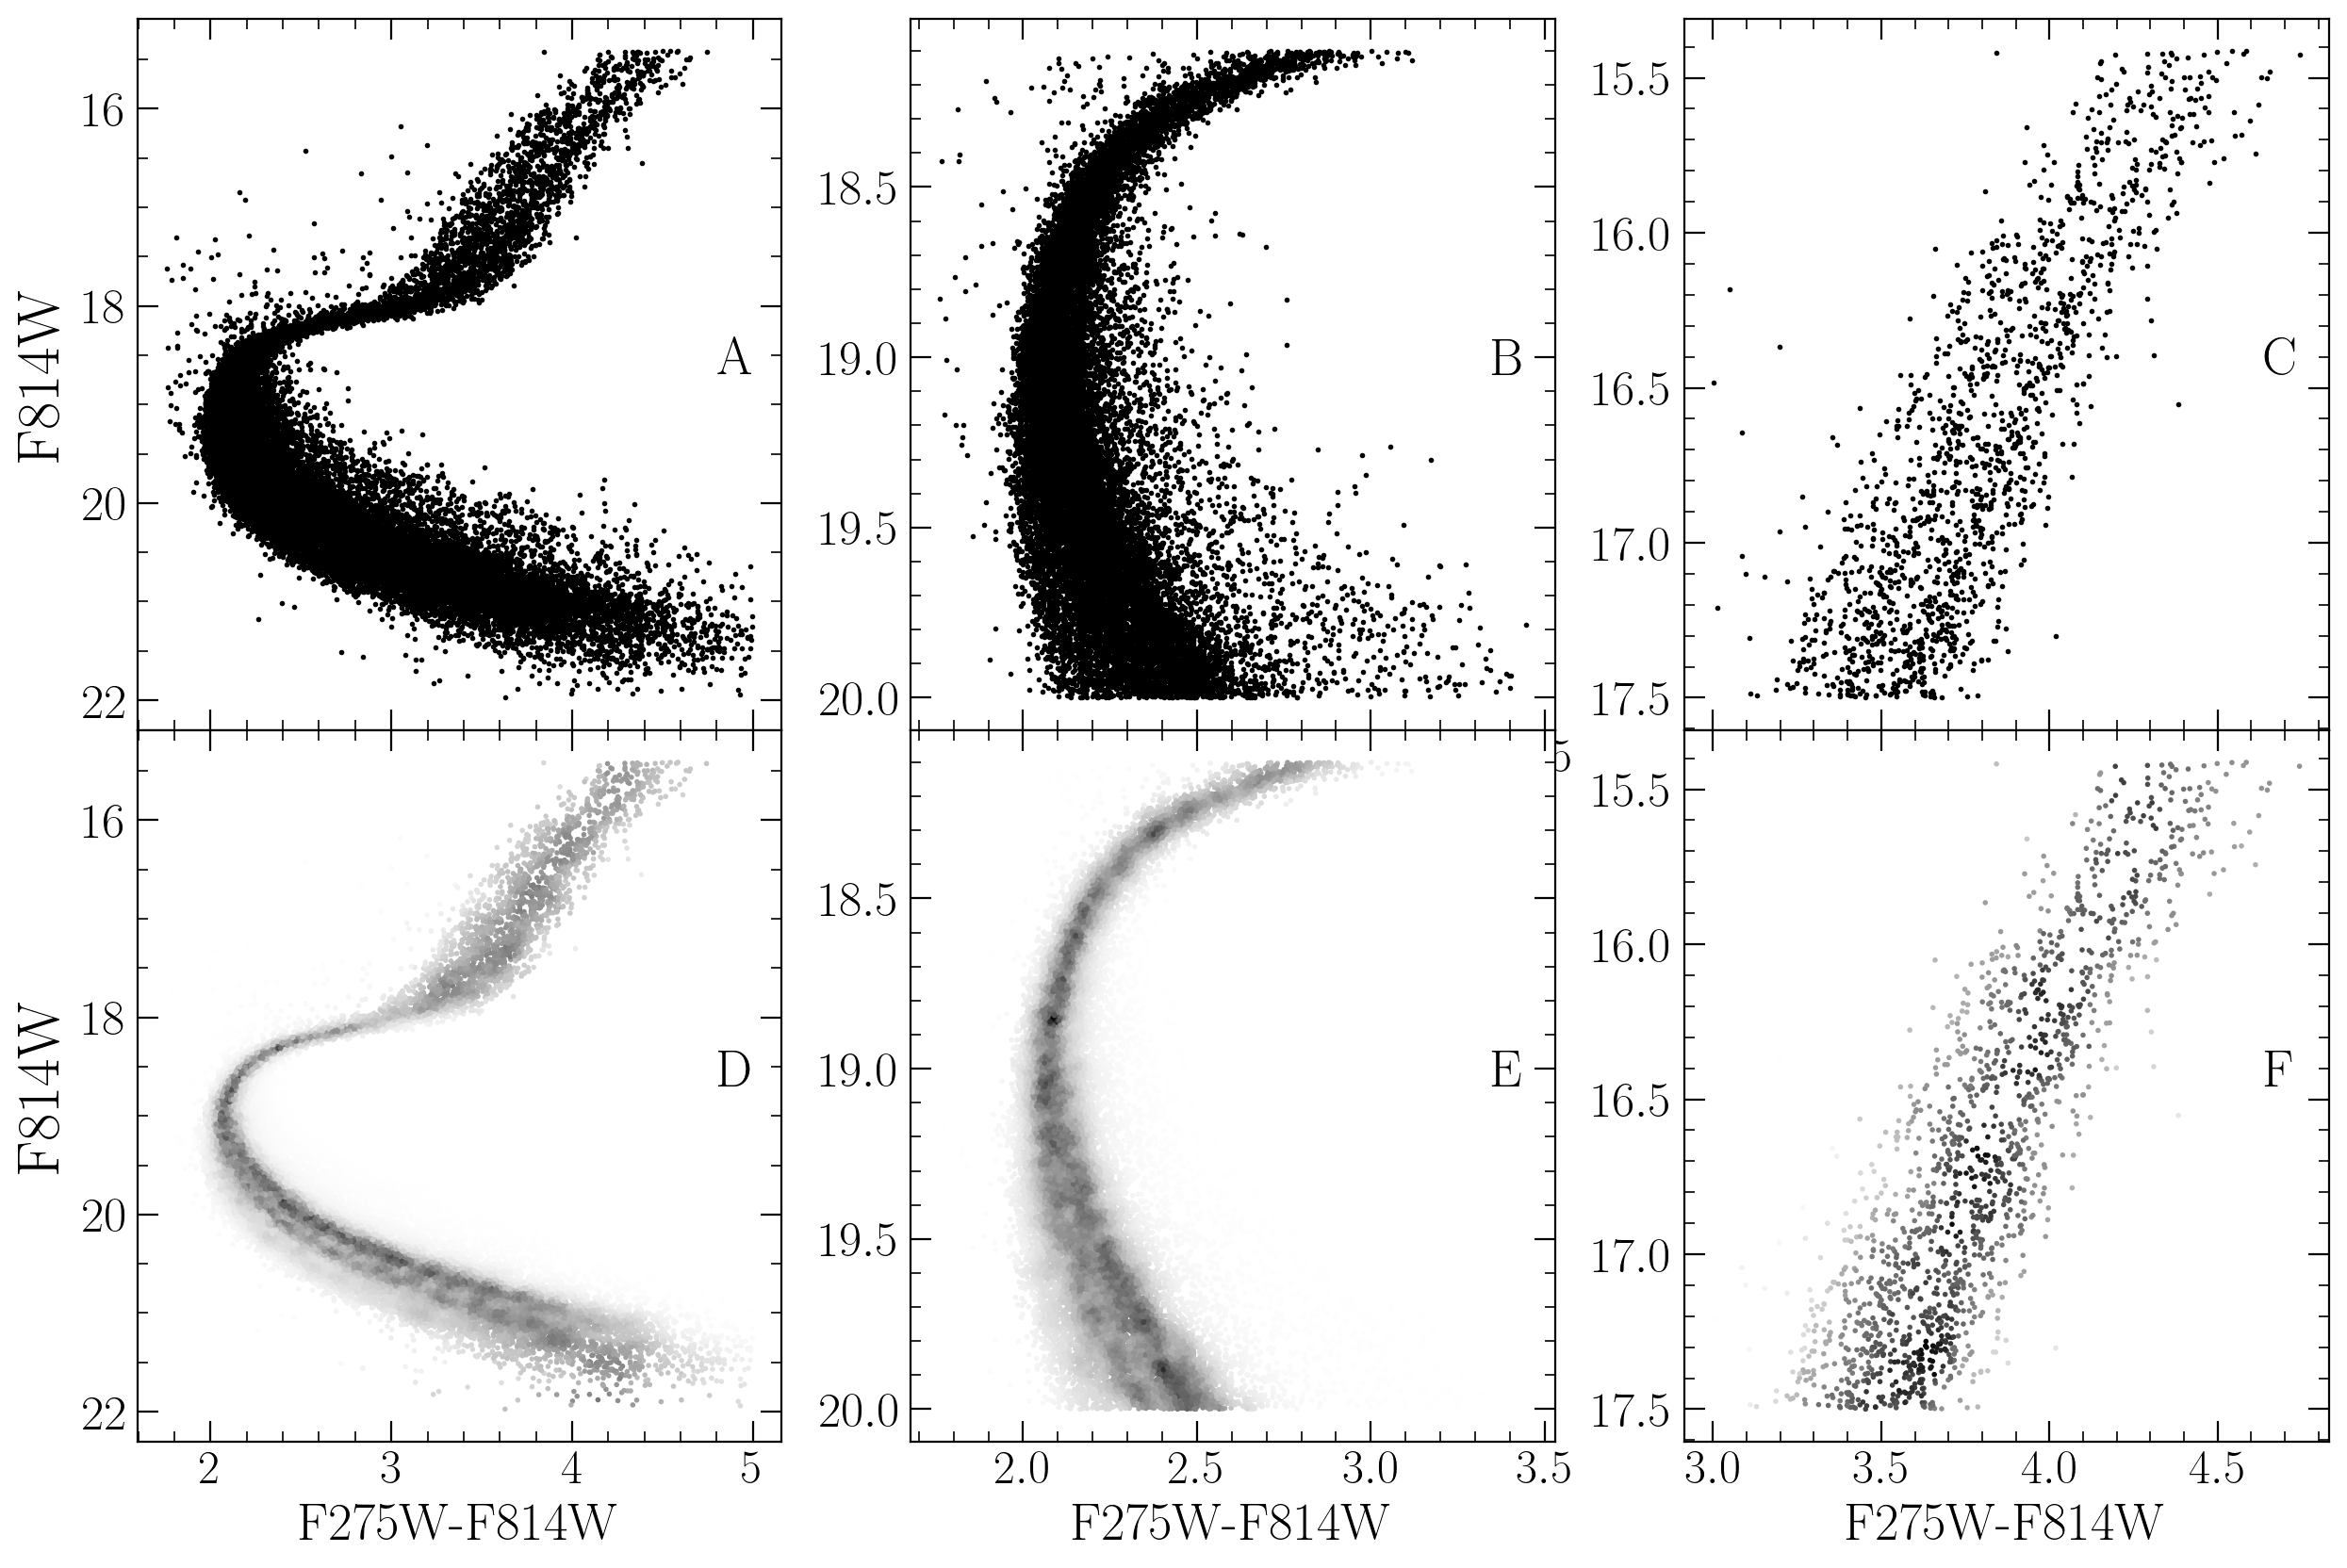
\includegraphics[width=0.9\textwidth]{figures/ngc2808/notebookFigures/DensityMapDemo.png}
  \caption{Figures in the top row are the raw CMD, while figures in the bottom
  row are colored by the density map.Density map demo showing density estimate
  over different parts of the evolutionary sequence. The left panel shows the
  density map over the entire evolutionary sequence, while the middle panel
  shows the density map over the main sequence and the right most panel shows
  the density map over the RGB. }
	\label{densityMapDemo}
\end{figure*}

\fidanka can now exploit this density map to fit a better fiducial line to the
data, as the density map is far more robust to outliers. There are multiple
algorithms we implement to fit the fiducial line to the color-density profile
in each magnitude bin (Figure \ref{densityBinsDemo}); they are explained in
more detail in the \fidanka documentation. However, of most relevance here is
the Bayesian Gaussian Mixture Modeling (BGMM) method. BGMM is a clustering
algorithm which, for some fixed number of n-dimensional Gaussian distributions,
$K$, determines the mean, covariance, and mixing probability (somewhat
analogous to amplitude) of each $k^{th}$ distribution, such that the local
lower bound of the likelihood of each star belonging strongly to a single
distribution is maximized. 

\begin{figure}
	\centering
	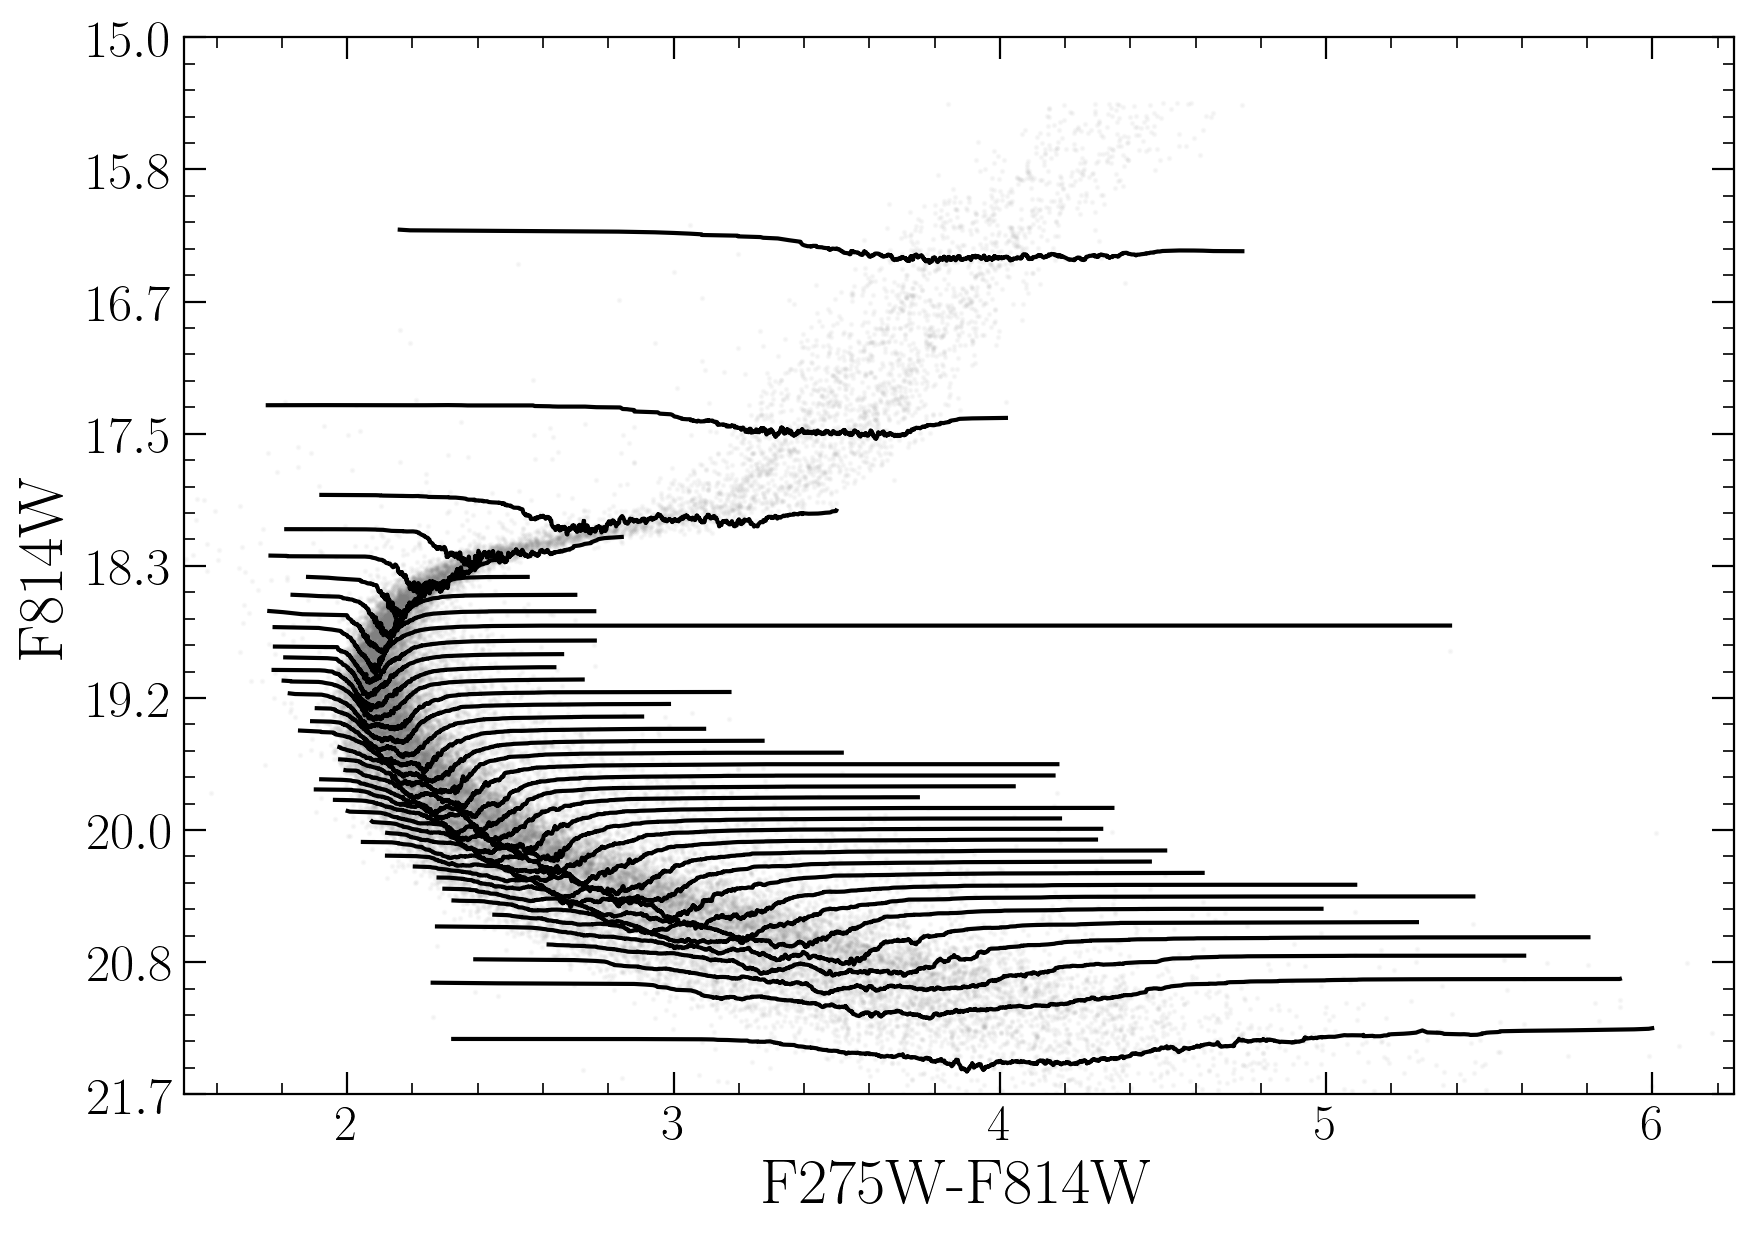
\includegraphics[width=0.85\textwidth]{figures/ngc2808/notebookFigures/DensityBinsDemo.png}
	\caption{CMD where point brightness is determined by local density. Lines show the
	density-color profile in each magnitude bin. In this figure adaptive
	binning targeted 1000 stars per bin}
	\label{densityBinsDemo}
\end{figure}

Maximization is performed using the Dirichlet process, which is a
non-parametric Bayesian method of determining the number of Gaussian
distributions, $K$, which best fit the data \citep{Ferguson1973, scikit-learn}.
Use of the Dirichlet process allows for dynamic variation in the number of
inferred populations from magnitude bin to magnitude bin. Specifically,
populations are clearly visually separated from the lower main sequence through
the turn off; however, at the turn off and throughout much of the subgiant
branch, the two visible populations overlap due to their extremely similar ages
\citep[i.e.][]{Jordan2002}. The Dirichlet process allows for the BGMM method to
infer a single population in these regions, while inferring two populations in
regions where they are clearly separated. More generally, the use of the
Dirichlet process removes the need for a prior on the exact number of
populations to fit. Rather, the user specifies a upper bound on the number of
populations within the cluster. An example bin (F814W = 20.6) is shown in
Figure \ref{fig:BGMMDist}.

\begin{figure*}
	\centering
	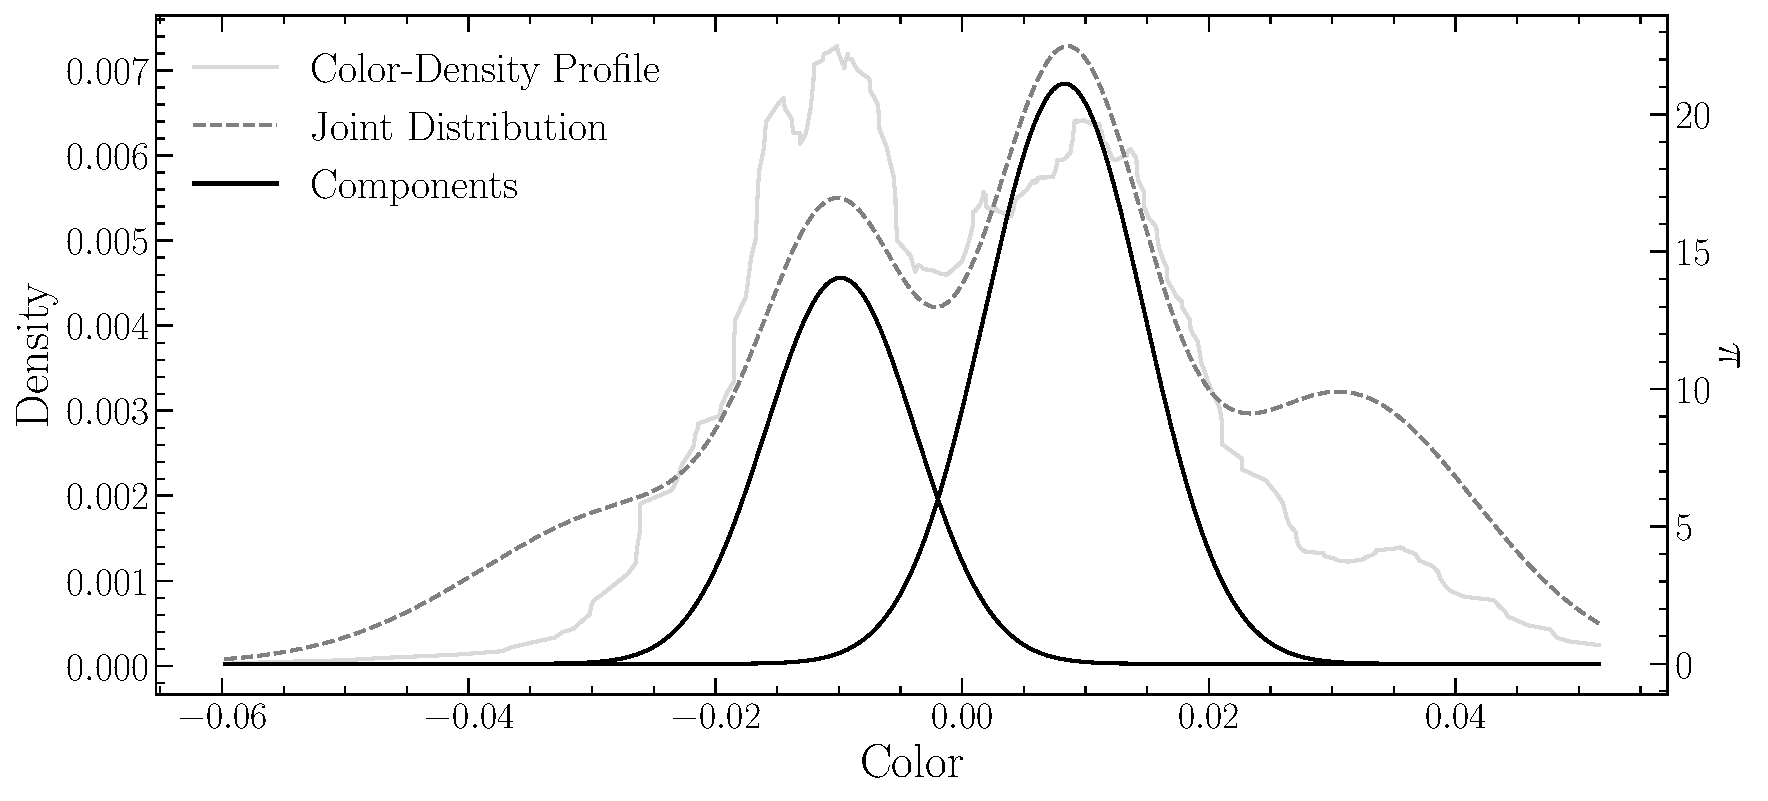
\includegraphics[width=0.9\textwidth]{figures/ngc2808/BGMMMixingBin.pdf}
	\caption{Example of BGMM fit to a magnitude bin. The grey line shows the
	underlying color-density profile, while the black dashed-line shows the
	joint distribution of each BGMM component. The solid black lines show the
	two selected components.}
	\label{fig:BGMMDist}
\end{figure*}

\fidanka's BGMM method first breaks down the verticalized CMD into magnitude
bins with uniform numbers of stars per bin (here we adopt 250). Any stars left
over are placed into the final bin. For each bin a BGMM model with a maximum of
5 populations is fit to the color density profile. The number of populations is
then inferred from the weighting parameter (the mixing probability) of each
population. If the weighting parameter of any $k^{th}$ components less than
{\color{blue}0.05}, then that component is considered to be spurious and
removed. Additionally, if the number of populations in the bin above and the
bin below are the same, then the number of populations in the current bin is
forced to be the same as the number of populations in the bin above. Finally,
the initial guess fiducial line is added back to the BGMM inferred line. Figure
\ref{fig:vertFit} shows the resulting fiducial line(s) in each magnitude bin
for both a verticalized CMD and a non verticalized CMD. In contrast to other
work in the literature where evidence for up to 5 distinct populations has been
found; we only find evidence for two stellar populations.

\begin{figure}
	\centering
	\includegraphics[width=0.65\textwidth]{figures/ngc2808/vertFit.png}
  \caption{Verticalized CMD (where the color of each data point is subtracted
  from the color of the fiducial line at that magnitude) where point brightness
  is determined by density (top). CMD where point brightness is determined by
  density, calculated fiducial lines are shown (bottom). The data used is from
  the Hubble Space Telescope UV Legacy Survey of Galactic Globular Clusters.}
	\label{fig:vertFit}
\end{figure}

This method of fiducial line extraction effectively discriminated between
multiple populations along the main sequence and RGB of a cluster, while
simultaneously allowing for the presence of a single population along the MSTO
and subgiant branch. 

We can adapt this density map based BGMM method to consider photometric
uncertainties by adopting a simple Monte Carlo approach. Instead of measuring
the fiducial line(s) a single time, \fidanka can measure the fiducial line(s)
many times, resampling the data with replacement each time. For each resampling
\fidanka adds a random offset to each filter based on the photometric
uncertainties of each star. From these $n$ measurements the mean fiducial line
for each sequence can be identified along with upper and lower bound confidence
intervals in each magnitude bin.

\subsection{Stellar Population Synthesis}
While not extensively used in this paper \fidanka can, in addition to measuring fiducial
lines, perform stellar population synthesise. \fidanka's population synthesis
module can generate synthetic stellar population from a set of MIST formatted
isochrones. This is of primary importance for binary population modeling. The
module is also used to generate synthetic CMDs for the purpose of testing the
fiducial line extraction algorithms against priors.

\fidanka uses MIST formatted isochrones \citep{Dotter2016} as input along
with distance modulus, B-V color excess, binary mass fraction, and bolometric
corrections. An arbitrarily large number of isochrones may be used to define an
arbitrary number of populations. Synthetic stars are samples from each
isochrone based on a definable probability (for example it is believed that
$\sim90\%$ of stars in globular clusters are younger population
\citep[e.g.][]{Suntzeff1996, Carretta2013}). Based on the metallicity, $\mu$, and E(B-V) of each
isochrone, bolometric corrections are taken from bolometric correction tables.
Where bolometric correction tables do not include exact metallicities or
extinctions a linear interpolation is performed between the two bounding
values. 

\subsection{Isochrone Optimization}
The optimization routines in \fidanka will find the best fit distance modulus,
B-V color excess, and binary number fraction for a given set of isochrones. If
a single isochrone is provided then the optimization is done by minimizing the
$\chi^2$ of the perpendicular distances between an isochrone and a fiducial
line. If multiple isochrones are provided then those isochrones are first used
to run stellar population synthesis and generate a synthetic CMD. The
optimization is then done by minimizing the $\chi^2$ of both the perpendicular
distances between and widths of the observed fiducial line and the fiducial
line of the synthetic CMD.


\subsection{Fidanka Testing}
In order to validate fidanka we have run an series of injection recovery tests
using \fidanka's population synthesis routines to build various synthetic
populations and \fidanka's fiducial measurement routines to recover these
populations. Each population was generated using the initial mass function
given in \citep{Milone2012} for the redmost population ($\alpha=-1.2$).
Further, every population was given a binary population fraction of 10\%,
distance uniformly sampled between 5000pc and 15000pc, and a B-V color excess
uniformly sampled between 0 and 0.1. Finally, each synthetic population was
generated using a fixed age  uniformlly sampled between 7 Gyr and 14 Gyr. An
example synthetic population along with its associated best fit isochrone are
shown in Figure \ref{fig:ValidationBestFit}.

\begin{figure}
  \centering
  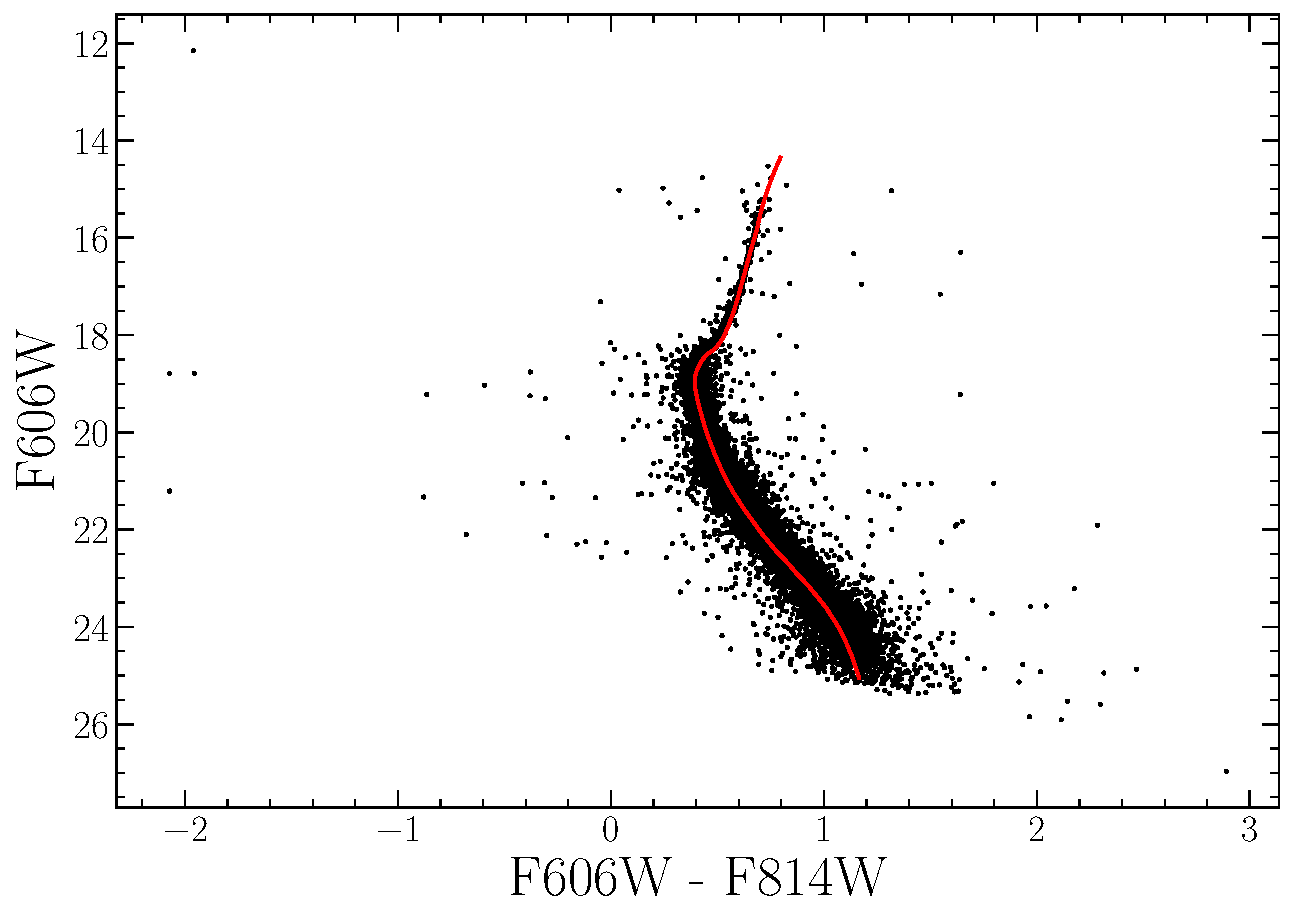
\includegraphics[width=0.85\textwidth]{figures/ngc2808/ExtractedIsoFit.pdf}
  \caption{Synthetic population generated by \fidanka at 10000pc with E(B-V) =
  0, and an age of 12 Gyr along with the best fitting isochrone. The best fit
  paremeters are derived to be $mu=15.13$, E(B-V)=0.001, and an age of 12.33
  Gyr.}
  \label{fig:ValidationBestFit}
\end{figure}

For each trial we use \fidanka to measure the fiducial line and then optimize
that fiducial line against the originating isochrone to estimate distance
modulus, age, and color B-V excess. Figure \ref{fig:validationDist} is built
from 1000 Monte-Carlo trials and shows the mean and width of the percent
error distributions for $\mu$, $A_{v}$, and age. In general \fidanka is able to
recover the distance modulus effectively with age and E(B-V) recovery falling in
line with other literature that does not consider the CMD outside of the main
sequence, main sequence turn off, sub giant, and red giant branches;
specifically, it should be noted that \fidanka is not setup to model the
horizontal branch.

\begin{figure}
  \centering
  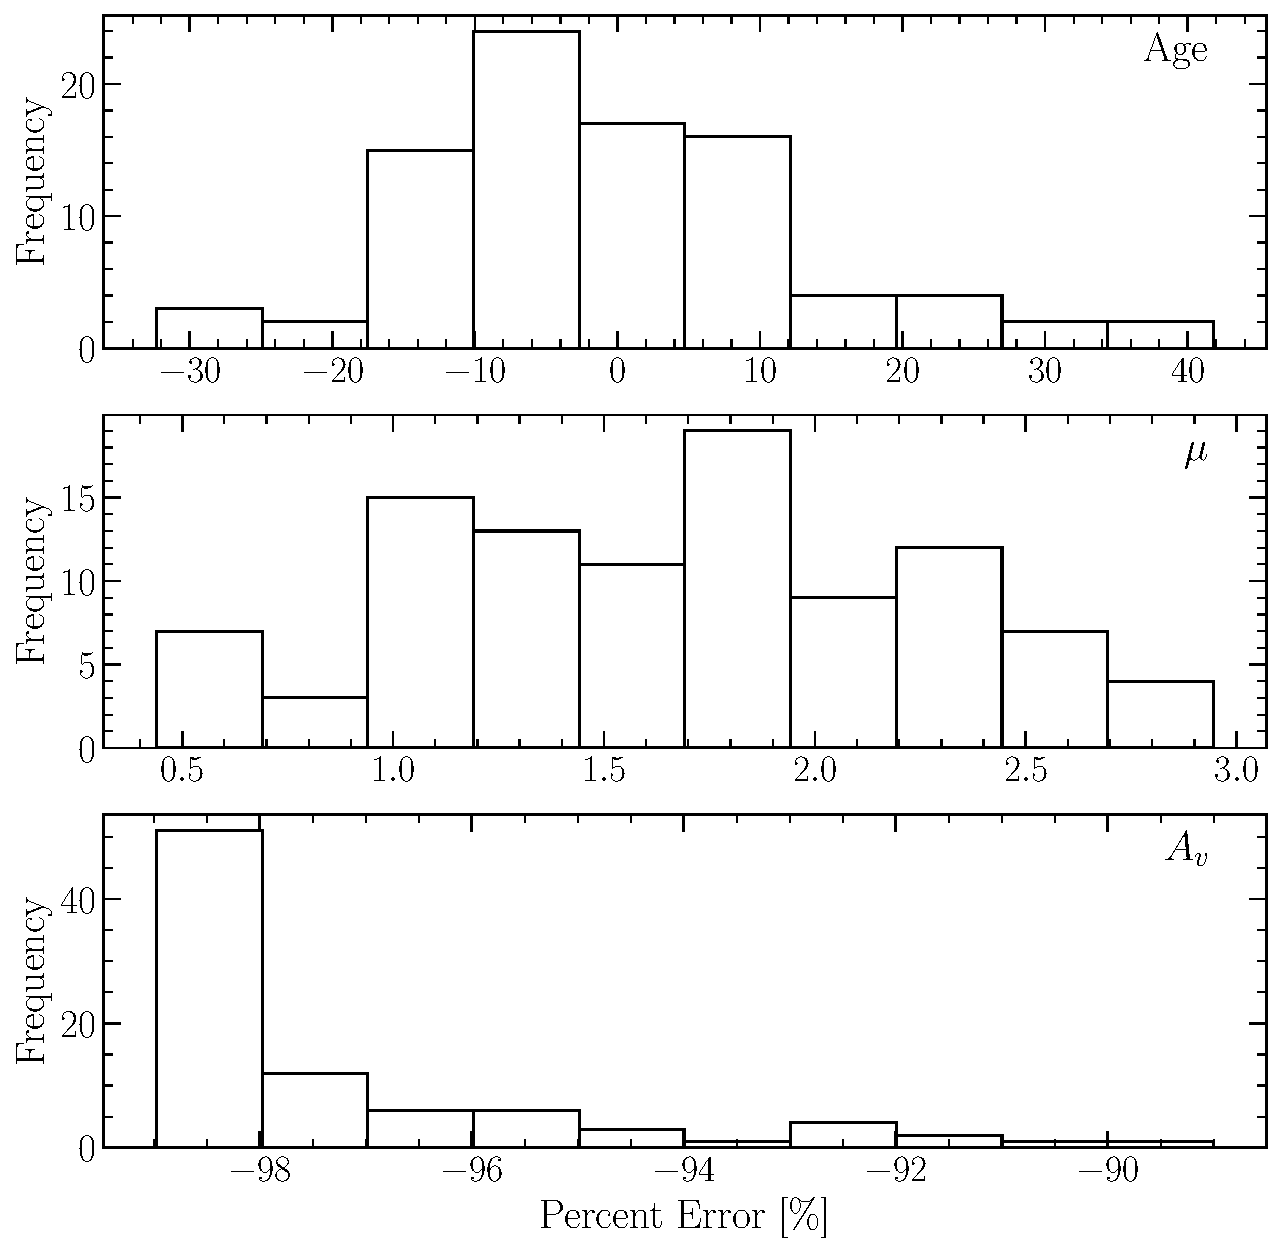
\includegraphics[width=0.85\textwidth]{figures/ngc2808/DistributionOfErrors.pdf}
  \caption{Percent Error distribution for each of the three derived parameters.
  Note that these values will be sensitive to the magnitude uncertainties of
  the photometry. Here we made use of the ACS artificial star tests to estimate
  the uncertainties.}
  \label{fig:validationDist}
\end{figure}
